\documentclass[xcolor={dvipsnames,svgnames}]{beamer}

\usepackage[utf8]{inputenc}
\usepackage[T1]{fontenc}
\usepackage[frenchb]{babel}

\usepackage{hyperref}
\usepackage{graphicx}
\graphicspath{ {./Images/} }

\usepackage{tikz}
\usetikzlibrary{shapes.geometric}
\usepackage{caption}
\usepackage{multirow}
\usepackage{array}

\usetheme{Madrid}

%https://tex.stackexchange.com/questions/173853/how-to-customize-colors-of-a-beamer-presentation

\setbeamercolor*{structure}{bg=PineGreen!20,fg=PineGreen}

\setbeamercolor*{palette primary}{use=structure,fg=white,bg=structure.fg}
\setbeamercolor*{palette secondary}{use=structure,fg=white,bg=structure.fg!75}
\setbeamercolor*{palette tertiary}{use=structure,fg=white,bg=structure.fg!50!black}
\setbeamercolor*{palette quaternary}{fg=white,bg=black}

\setbeamercolor{section in toc}{fg=black,bg=white}
\setbeamercolor{alerted text}{use=structure,fg=structure.fg!50!black!80!black}

\setbeamercolor{titlelike}{parent=palette primary,fg=structure.fg!50!black}
\setbeamercolor{frametitle}{bg=gray!10!white,fg=PineGreen}

\setbeamercolor*{titlelike}{parent=palette primary}

\usefonttheme{serif}


\title{Présentation d'article}
\subtitle{Light Pattern: Writing Code with Photographs}
\author{Luchino Allix-Lastrego}
\institute{6251 - Art algorithmique}
\date{20 Mars 2025}

\makeatletter
\setbeamertemplate{footline}{%
  \leavevmode%
  \hbox{%
    \begin{beamercolorbox}[wd=.37\paperwidth,ht=2.25ex,dp=1ex,center]{title in head/foot}%
      \usebeamerfont{title in head/foot}\insertshorttitle  % Affiche le titre
    \end{beamercolorbox}%
	\begin{beamercolorbox}[wd=.26\paperwidth,ht=2.25ex,dp=1ex,center]{author in head/foot}%
		\usebeamerfont{author in head/foot}%
		\ifx\insertsection\empty
		Introduction
		\else
		  \insertsection  % Affiche la section actuelle
		\fi
	\end{beamercolorbox}%
    \begin{beamercolorbox}[wd=.37\paperwidth,ht=2.25ex,dp=1ex,right]{date in head/foot}%
      \usebeamerfont{date in head/foot}\insertshortdate{}\hspace*{2em}  % Affiche la date
      \insertframenumber{} / \inserttotalframenumber  % Affiche le numéro de diapositive
      \hspace*{2ex}
    \end{beamercolorbox}}%
  \vskip0pt%
}
\makeatother

\begin{document}

\begin{frame}
	\titlepage
	\begin{center}
		
\includegraphics[scale=.075]{logo_diro.png}

		\vspace{0.3cm}

		Université de Montréal\\
		Département d'informatique et de recherche opérationnelle\\

	\end{center}
\end{frame}

\begin{frame}{Table des matières}
	\tableofcontents
\end{frame}

\section{Introduction}
\begin{frame}
	\centering
	\Large Introduction
\end{frame}

\subsection{Article}
\begin{frame}{Article}
	\begin{block}{General information}
		\begin{itemize}
			\item Titre : \href{https://history.siggraph.org/wp-content/uploads/2018/04/2015_Temkin_LightPattern.pdf}{Light Pattern: Writing Code with Photographs}
			\item Auteur : \href{https://danieltemkin.com/}{Daniel Temkin}
			\item Publication : 2015, sur \href{https://history.siggraph.org/}{ACMSIGGRAPH}
		\end{itemize}
	\end{block}

	\hfill

	\begin{center}
		
\includegraphics[scale=.3]{ACM.png}
	\end{center}
	
\end{frame}

\subsection{Objectif}
\begin{frame}{Objectif}
	\begin{block}{Concept principal}
		Écrire du code avec des photos au lieu de text.
	\end{block}

	\hfill
	
	\begin{itemize}
		\item Emphase sur comment on code plutôt que ce qu'on code
		\item Remet en question la notion de langage de programmation
		\item Évoque les langages de programmation comme médium pour l'art
	\end{itemize}
\end{frame}


\section{Fonctionnement}
\begin{frame}
	\centering
	\Large Fonctionnement
\end{frame}

\subsection{Syntaxe}
\begin{frame}{Syntaxe et particularités}
	\begin{itemize}
		\item Code source {\tt =>} suite de fichier JPEGs dans un directory
		\item Exécution du code {\tt =>} lecture des fichiers par ordre alphabétique
		\item Changement d'image {\tt =>} code de trois chiffre qui fait quelque chose 
		\item Basé sur {\tt Java} et {\tt C\#} (écrit en {\tt C\#})
		\item Stack based
		\item vocabulary-oriented
	\end{itemize}
\end{frame}

\begin{frame}{Changement d'image}
	En passant d'une image à une autre on note la différence de :
	\begin{itemize}
		\item aperture
		\item couleur
		\item shutter
	\end{itemize}
	
	\hfill

	Par exemple pour l'aperture :
	\begin{itemize}
		\item darker : 0
		\item no change : 1
		\item brighter : 2
	\end{itemize}
\end{frame}

\subsection{Démonstration}
\begin{frame}{Démonstration}
	
	Hello world :
	\begin{center}
		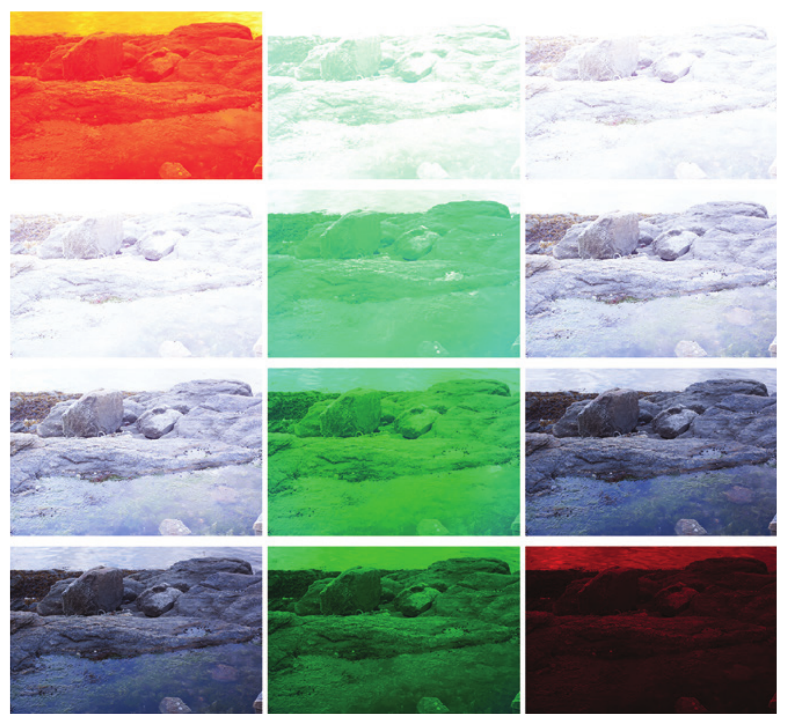
\includegraphics[scale=.35]{hello.png}
	\end{center}
	
\end{frame}

\begin{frame}{Exécution}
	
	\begin{center}
		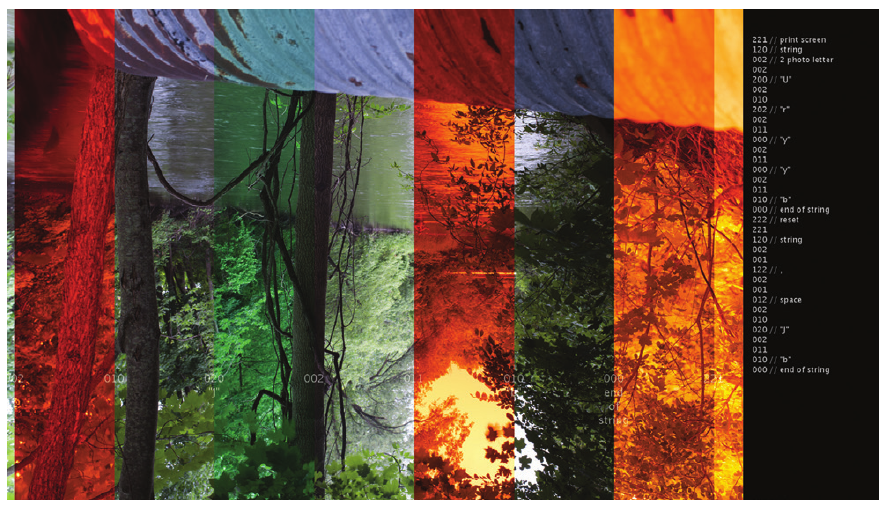
\includegraphics[scale=.45]{world.png}
	\end{center}

	Il aura fallut 51 photos pour écrire le programme.

	Lien vers la vidéo d'exécution de \href{https://vimeo.com/102076781}{\emph{"Hello, World!"}}
\end{frame}

\section{Questionnements}
\begin{frame}
	\centering
	\Large Questionnements
\end{frame}

\begin{frame}{Questionnements}
	\begin{center}
		Pourquoi définir un langage de programmation (quasiment) inutilisable ?
	\end{center}
\end{frame}

\subsection{Esolang}
\begin{frame}{Esolang}
	\begin{block}{\href{https://en.wikipedia.org/wiki/Esoteric_programming_language}{Esoteric programming language} / langage de programmation exotique  :}
		\begin{itemize}
			\item tester les limites de la création de langages de programmation
			\item exercice intellectuel
			\item blague
		\end{itemize}
	\end{block}
\end{frame}

\begin{frame}{Exemples}
	\begin{block}{Brainfuck}
		Seulement 8 instructions (variantes : Whitespace, jsfuck)
		\begin{center}
			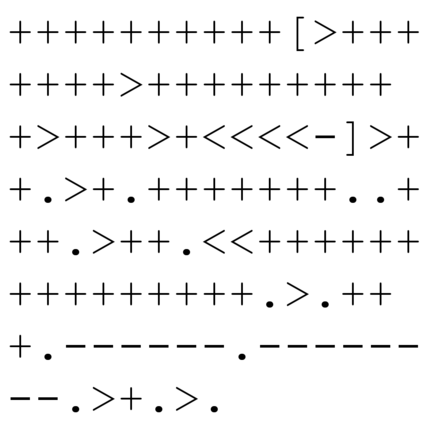
\includegraphics[scale=.25]{brainfuck.png}
		\end{center}
	\end{block}
	\begin{block}{Whenever}
		Les lignes de code sont comme des cases de todo list, l'interpréteur les exécute dans l'ordre qu'il souhaite
	\end{block}
\end{frame}

\begin{frame}
	\begin{block}{Malboge}
		Il a fallut 3 ans pour trouver comment écrire \emph{"Hello, World"}.	
		\begin{center}
			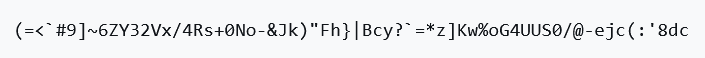
\includegraphics[scale=.6]{malboge.png}
		\end{center}
		Créateur : \emph{"pushing the boundaries of programming, but not in useful directions"}
	\end{block}
	
	\begin{block}{Piet}
		Écrire avec des bitmap :
		\begin{center}
			
\includegraphics[scale=.5]{Piet.png}
		\end{center}
	\end{block}
\end{frame}

\subsection{Liens avec l'art}
\begin{frame}{Liens avec l'art}
	\begin{block}{\href{https://fr.wikipedia.org/wiki/Oulipo}{Oulipo}}
		L'ouvroir de littérature potentielle :
		\begin{itemize}
			\item découvrir de nouvelles potentialités du langage
			\item moderniser l'expression à travers des jeux d'écriture
			\item Fondé sur le principe que la contrainte provoque et incite à la recherche de solutions originales
		\end{itemize}

		Queneau (un des fondateurs) : \emph{"to become the rats who build the labyrinth from which they will try to escape"}

		\begin{center}
			
\includegraphics[scale=.2]{oulipo.png}
		\end{center}
	\end{block}
\end{frame}

\begin{frame}
	\begin{block}{\href{https://fr.wikipedia.org/wiki/Fluxus}{Fluxus}}
		\begin{itemize}
			\item mouvement artistique né dans les années 1960
			\item anti-art
			\item non-mouvement
			\item art-distraction
		\end{itemize}
	\end{block}

\end{frame}

\section{Conclusion}
\begin{frame}{Conclusion}
	Light Pattern s'inscrit dans une optique de rassembler esolang avec une dynamique artistique telle que Oulipo et Fluxus.
\end{frame}

\end{document}
